\documentclass[11pt]{article}
\setlength{\headheight}{14pt}

% ---------------------------------------------------------------------
% Packages
% ---------------------------------------------------------------------
\usepackage[margin=1in]{geometry}
\usepackage{amsmath, amssymb, amsthm}
\usepackage{pdflscape}
\usepackage{mermaid}
\usepackage{booktabs}
\usepackage{graphicx}
\usepackage{xcolor}
\usepackage{enumitem}
\usepackage{listings}
\usepackage{algorithm}
\usepackage{algpseudocode}
\usepackage{pgfplots}
\usepackage{fancyhdr}
\usepackage{float}
\usepackage{placeins}
\usepackage[hidelinks]{hyperref}

\pgfplotsset{compat=1.16}

% ---------------------------------------------------------------------
% Course info (edit these per project)
% ---------------------------------------------------------------------
\newcommand{\studentname}{Riley Herchert, Shelbe Yousey, Casen Parmer}
\newcommand{\instructorname}{Dr. Yessick}
\newcommand{\taname}{Lucas Hasting}
\newcommand{\coursename}{CS 201}
\newcommand{\projectname}{Project \#3}

% ---------------------------------------------------------------------
% Handy macros
% ---------------------------------------------------------------------
\newcommand{\todo}[1]{\textcolor{red}{[#1]}}
\newcommand{\Oh}{\mathcal{O}}

% ---------------------------------------------------------------------
% Code listing style
% ---------------------------------------------------------------------
\lstset{
  language=C++,
  basicstyle=\ttfamily\footnotesize,
  keywordstyle=\color{blue!70!black},
  commentstyle=\color{green!40!black},
  numbers=left, numberstyle=\tiny, numbersep=6pt,
  frame=single, breaklines=true, columns=fullflexible,
  showstringspaces=false
}

% Plain-output style: use as \begin{lstlisting}[style=outputstyle]
\lstdefinestyle{outputstyle}{
  basicstyle=\ttfamily\small,
  breaklines=true,
  backgroundcolor=\color{gray!10},
  frame=single,
  numbers=none,
  columns=fullflexible
}

% ---------------------------------------------------------------------
% Theorem environments
% ---------------------------------------------------------------------
\theoremstyle{plain}
\newtheorem{theorem}{Theorem}
\newtheorem{lemma}{Lemma}
\theoremstyle{definition}
\newtheorem{claim}{Claim}

% ---------------------------------------------------------------------
% Header / footer
% ---------------------------------------------------------------------
\pagestyle{fancy}
\fancyhf{}
\lhead{\coursename{} -- \projectname}
\rhead{\studentname}
\cfoot{\thepage}

% ---------------------------------------------------------------------
% Title
% ---------------------------------------------------------------------
\title{\coursename{} -- \projectname{} Report}
\author{\studentname\\
        Instructor: \instructorname \\
        TA: \taname}
\date{\today}

\begin{document}
\maketitle

\section{UML Diagram}

\begin{figure}[H]
\MermaidAdjustBoxOpts{max width=\linewidth, max totalheight=0.6\textheight, center}
\begin{mermaid}
%%{init: {"theme": "neutral", "look": "classic"}}%%
classDiagram
    direction TB

    class Person {
        #name: string
        #age: int
        #birthdate: string
        #id: int
        +Person(name: string, age: int, birthdate: string)
        +~Person()
        +getName() string
        +getAge() int
        +getBirthdate() string
        +getID() size_t
    }

    class Doctor {
        -skill: int
        -available: bool
        -startTime: int
        -endTime: int
        +Doctor(name: string, age: int, birthdate: string, skill: int, available: bool, startTime: int, endTime: int)
        +getSkill() int
        +isAvailable() bool
        +setAvailability(avail: bool) void
        +getStartTime() int
        +getEndTime() int
    }

    class Patient {
        -condition: int
        -status: PatientStatus
        -eta: int
        -arrivalTime: int
        +Patient(name: string, age: int, birthdate: string, condition: int, arrivalTime: int)
        +seeDoctor(eta: int) void
        +getStatus() PatientStatus
        +getETA() int
        +getArrivalTime() int
        +getCondition() int
        +updateStatus(newStat: PatientStatus) void
    }

    class PatientStatus {
        <<enumeration>>
        SCHEDULED
        WAITING
        IN_VISIT
        FAILED_TO_TREAT
        DISCHARGED
    }

    namespace bst {
        class BstNode["Node"] {
            +value: Doctor#42;
            +key: int
            +left: Node#42;
            +right: Node#42;
            +parent: Node#42;
            +Node(value: Doctor#42;, key: int)
        }
        class BstTree["Tree"] {
            +root: Node#42;
            +Tree()
            +~Tree()
            +insert(newNode: Node#42;) void
            +deleteSubtree(node: Node#42;) void
            +empty() bool
            +max() Doctor#42;
            +remove(node: Node#42;) void
            +find(value_id: size_t, skill_rank: int) Node#42;
        }
    }

    namespace b_tree {
        class BNode["Node"] {
            +values: vector~Person#42;~
            +keys: vector~size_t~
            +children: vector~Node#42;~
            +leaf: bool
            +Node(value: Person#42;, key: size_t)
            +Node(isLeaf: bool)
            +insertValueKeyPair(value: Person#42;, key: size_t, i: int) void
            +fillWithValues(fullNode: Node#42;, t: int) void
            +shrinkNode(t: int) void
        }
        class BTree {
            +root: Node#42;
            +t: int
            +BTree(degree: int)
            +~BTree()
            +splitChild(parent: Node#42;, index: int) void
            +insertNonFull(node: Node#42;, value: Person#42;, key: size_t) void
            +insert(value: Person#42;, key: size_t) void
            +searchHelper(node: Node#42;, key: size_t) Person#42;
            +search(key: size_t) Person#42;
            +inorderHelper(node: Node#42;, out: vector~Person#42;~&) void
            +inorder() vector~Person#42;~
            +deleteTree(node: Node#42;) void
        }
    }

    namespace maxHeap {
        class MaxHeap["maxHeap&lt;T, Cmp&gt;"] {
            -items: vector~T#42;~
            -cmp: Cmp
            +push(item: T#42;) void
            +top() T#42;
            +pop() void
            +empty() bool
        }
    }

    class Simulation {
        -TIME_LIMIT: int = 30$
        -records: b_tree::BTree
        -patientQueue: maxHeap&lt;Patient&gt;
        -shiftDoctors: bst::Tree
        -offShiftDoctors: maxHeap&lt;Doctor&gt;
        -currentPairings: vector~pair&lt;Doctor#42;, Patient#42;&gt;~
        -discharged: vector~Patient#42;~
        -failed: vector~Patient#42;~
        -time: int
        -paired: bool
        -dischargePatients() void
        -startShifts() void
        -createPairings() void
        -treatmentTime(p: Patient#42;, d: Doctor#42;) int
        +Simulation()
        +Simulation(startTime: int)
        +step() void
        +stepPhase() void
        +addPerson(patient: Patient) void
        +addPerson(doctor: Doctor) void
        +findPatient(name: const string&, age: int, birthdate: const string&) Patient#42;
        +findDoctor(name: const string&, age: int, birthdate: const string&) Doctor#42;
        +getTime() int
        +isPaired() bool
        +isOnShift(d: Doctor#42;) bool
        +getWaiting() vector~Patient#42;~
        +getDoctors() vector~Doctor#42;~
        +getUpcomingCount() int
        +patientOf(d: Doctor#42;) Patient#42;
        +getPairings() const vector~pair&lt;Doctor#42;, Patient#42;&gt;~&
        +getDischarged() const vector~Patient#42;~&
        +getFailed() const vector~Patient#42;~&
    }

    class dataController {
        <<namespace>>
        +loadData(sim: Simulation&, numPatients: int, numDoctors: int, enableTestHarness: bool)$ void
        +generatePatient()$ Patient
        +generateDoctor()$ Doctor
    }

    class testHarness {
        <<free functions>>
        +runAllTests()$ void
        +printTestResult(success: bool, name: string, desc: string)$ void
    }

    Person <|-- Doctor
    Person <|-- Patient
    Patient --> PatientStatus : status

    BstTree "1" *-- "0..*" BstNode : root
    BstNode --> BstNode : left / right / parent
    BstNode --> Doctor : value

    BTree "1" *-- "1..*" BNode : root
    BNode --> BNode : children
    BNode --> "0..*" Person : values

    Simulation *-- BTree : records
    Simulation *-- "2" MaxHeap : patientQueue / offShiftDoctors
    Simulation *-- BstTree : shiftDoctors
    Simulation o-- "0..*" Patient : discharged / failed / pairings
    Simulation o-- "0..*" Doctor : pairings

    dataController ..> Simulation : loads
    dataController ..> Patient : creates
    dataController ..> Doctor : creates
\end{mermaid}
\caption{UML class diagram of the hospital simulation.}
\label{fig:uml}
\end{figure}

\section{Implementation Details}

As demonstrated above, the process of simulation is handled by a \texttt{Simulation} class. This is to ensure consistent implementation across both our GUI component and the test harness.

The simulation class owns multiple data structures, using the CLRS implementations as a base and modifying them to fit our needs. A B-tree is used for storing patient and doctor records. Max heaps are used for both the patient queue and off-shift doctors. Custom comparison operators were defined in \texttt{keys.h} to support our implementation. The patient with the earliest arrival time should be treated first. Similarly, the doctors with the earliest shift start times should be at the top of their max heap. We also used a binary search tree for the on-shift doctors, sorted by skill level. Since doctors with higher skill levels treat patients faster, the most patients can be seen by funneling patients towards high skill doctors. Generic vectors are used for doctor-patient pairings, as well as the list of discharged and failed patients.

Our B-tree uses a minimum degree of $t = 10$, so every node except the root holds between 9 and 19 keys and has up to 20 children. We chose this value to balance the tree's height against the work done inside each node. A larger $t$ makes the tree shallower, but our search and insert scan each node's keys one by one, so very large nodes would make each step slower. A smaller $t$ makes nodes cheap to scan, but the tree gets taller and splits happen more often. With $t = 10$, a tree of height $h$ can hold up to $(2t)^{h+1} - 1$ records. That means our default dataset of 110 people (100 patients and 10 doctors) fits in just two levels, and even 7{,}999 records would need only three. A lookup therefore touches at most two or three nodes, splits are rare during data loading, and the tree can grow well past our test data without losing that shallow shape.

The general flow of our implementation as follows:
\begin{enumerate}
  \item The makefile is used to select between the GUI and test harness execution.
  \begin{enumerate}
    \item If the test harness is used, tests are automatically executed and output to console.
    \item If the GUI is used, the SFML window launches.
    \item Both executions use a simulation class with predefined parameters.
  \end{enumerate}
  \item The \texttt{datacontroller} class is used to load patient and doctor data into the simulation.
  \item In each in minute (step), the following processes occur:
  \begin{enumerate}
    \item Discharge patients: patients who have completed their appointment (eta passed) are discharged from the hospital. If the doctor is still on shift, they are returned to the BST.
    \item Start shifts: the top of the max heap is checked, and any doctor who is now on shift is removed from the heap and placed in the BST.
    \item Create pairings: the top of the max heap (patient queue) is checked, and any patient who has now arrived is checked to confirm they are within the allotted time frame. If not, they are marked as failed. Otherwise, we attempt to find the highest-skilled, unpaired, on-shift doctor and move both the doctor and patient into a seperate vector. 
  \end{enumerate}
\end{enumerate}

\begin{figure}[h]
    \centering
    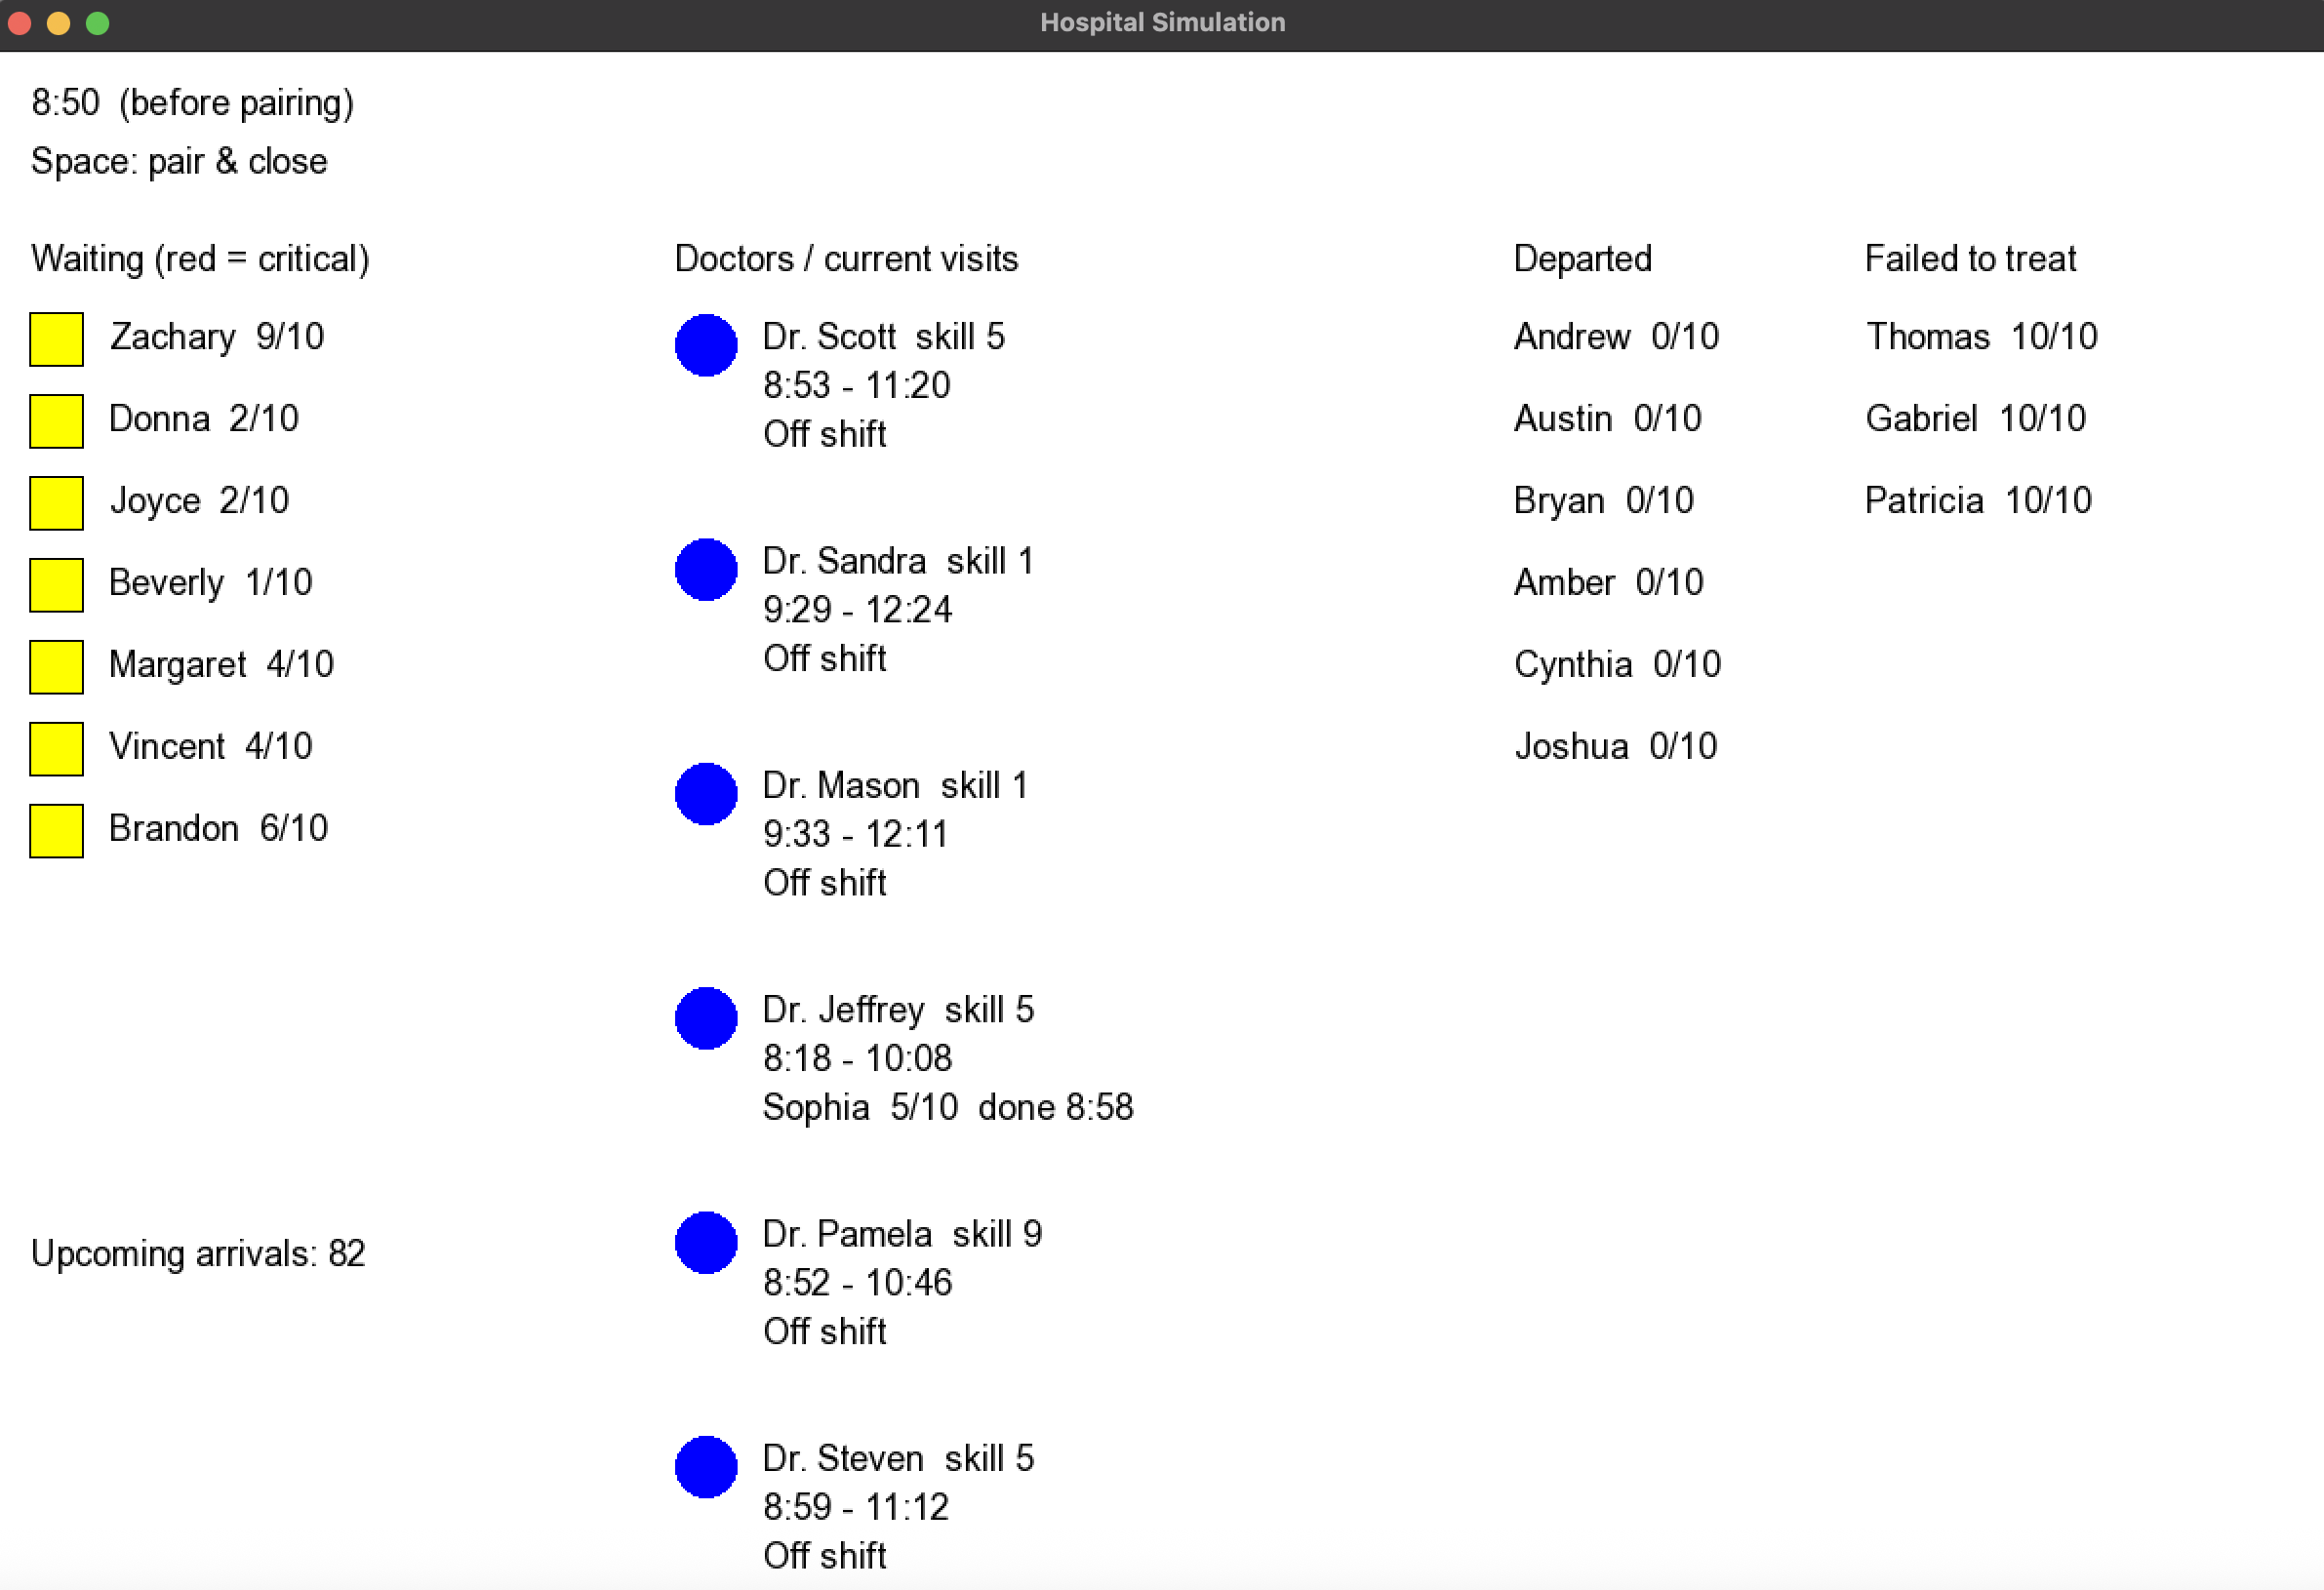
\includegraphics[width=0.8\textwidth]{demo}
    \caption{A screenshot demonstrating GUI functionality.}
\end{figure}

\section{Task Distribution}

\begin{enumerate}
  \item Riley Herchert
  \begin{enumerate}
    \item Code comments and documentation
    \item GUI implementation
    \item Test harness implementation
    \item Class implementation
    \item Data structure implementations
  \end{enumerate}
  \item Shelbe Yousey
  \begin{enumerate}
    \item Data structure refactors
    \item GUI refactors
    \item Class implementation
  \end{enumerate}
  \item Casen Parmer
  \begin{enumerate}
    \item Final report
    \item Class refactors
    \item Repo organization
    \item Data controller implementation
    \item Simulation implementation
  \end{enumerate}
\end{enumerate}

\end{document}
